\documentclass[reprint,amsmath,amssymb,aps]{revtex4-2}

% importing packages
% \usepackage{multicol}  % multiple columns
% \usepackage[utf8]{inputenc}  % input encoding
% % \usepackage{multirow} 		% for tables
% % \usepackage[italicdiff]{physics}  % physics
% % \usepackage{longtable}
% % \usepackage{float}  % floating figures
\usepackage{gensymb}  % math symbols
\usepackage{indentfirst}  % indent first line of paragraph
\usepackage{fancyvrb}  % verbatim
\usepackage{mathtools}  % math
\usepackage{xfrac}   % fractions
\usepackage[center]{caption}  % centering captions
\usepackage{amsmath}  		% for math symbols
\usepackage{physics} 		% for physics symbols
\usepackage{amssymb} 		% for math symbols
\usepackage{hyperref}  		% for hyperlinks
\usepackage{graphicx}  % adding pictures
\usepackage{dcolumn}
\usepackage{bm}


% defining new commands
\newcommand{\angstrom}{\textup{\AA}}  % angstrom
\DeclareMathOperator{\taninv}{tan^{-1}}
% \DeclareUnicodeCharacter{2212}{-}
\setlength{\columnsep}{0.5cm}  % column separation

% defining graphics path
% \graphicspath{ {./images/} }

% the next 5 lines help in removing the ugly
% boxes around links and making them look better
\hypersetup{
	colorlinks = true,
	urlcolor = black,
	linkcolor = black,
	citecolor = black,
}

\begin{document}

    \title{Seelab Introduction (Expt 9)}

    \author{Aritra Mukhopadhyay}
    \affiliation{
        National Institute of Science Education and Research\\
        Bhubaneswar, Odisha 751005, India\\
        3rd year, Integrated M.Sc. Physics\\
        Roll No.: 2011030
    }
    \date{\today}

    \begin{abstract}
	This experiment involved the construction and analysis of digital-to-analog converter (DAC) and analog-to-digital converter (ADC) circuits using integrated circuits. By sampling an input AC signal and passing it through a series of ADC and DAC, we were able to observe and verify that the output analog voltage is approximately equal to the input signal. We also studied the working and pin diagram of the ICs, and discussed the importance of sampling in these circuits. Overall, the experiment provided valuable insights into the operation and applications of DAC and ADC circuits.
\end{abstract}

    \maketitle

    \section{Experiments}
        \begin{itemize}
            \item Transistor characteristics
            \item Astable multivibrator with IC 555
            \item EM induction to determine magnetic moment are mandatory 
        \end{itemize}
    \section{Theory}
    \subsection{Magnetoresistance}
		Under the influence of a magnetic field, the resistance of some materials change significantly. This effect is popularly known as magnetoresistance of the material. This effect can be observed due to the fact that the drift velocity of the carriers is not same. In the presence of the Magnetic field, the carriers drift in the direction of the field. In this condition, the hall voltage compensates the lorentz force for carriers with average velocity. The slower carriers are overcompensated and the faster carriers are undercompensated. This disturbs the flow of electrons along the direction of flow of current; hence reducing the mean free path and increasing the resistance of the material. In this condition, the hall voltage is given by the formula:
		
		$$V = E_yt = |v\times H|$$

		where $E_y$ and $H$ are the electric field and the magnetic fields, $t$ is the thickness of the sample, and $v$ is the drift velocity of the carriers.

		The change in resistivity $\Delta\rho$ is positive for both magnetic field parallel $\Delta \rho_\parallel$ and transverse $\Delta \rho_T$ to the current direction with $\rho_T>\rho_\parallel$. There are three different kinds of magnetoresistance, depending on the structure of the electron orbitals at the Fermi surface:

		\begin{enumerate}
			\item The magnetic field has the effect of raising the cyclotron frequency of the electron in its confined orbit in metals with closed Fermi surfaces where the electrons are restricted to their orbit in k-space.
			\item The magnetoresistance for metals with an equal number of electrons and holes rises with magnetic field up to the highest observed fields and is unaffected by crystallographic orientation. These materials include bismuth.
			\item In some crystallographic orientations, Fermi surfaces with open orbits will show significant magnetoresistance for applied fields, but the resistance will saturate in other crystallographic directions where the orbits are closed.
		\end{enumerate}

	\subsection{Hall Effect}
		This effect was discovered by Edwin Hall in 1879. This is the production of a voltage across a conductor when an electric current is passed through it in the presence of a magnetic field. This results in the separation of charge carriers into two regions, one with positive charge and the other with negative charge. This will result in an electric field perpendicular to both the current and the magnetic field (in the $\vec{H}\times\vec{I}$ direction). 

		\begin{equation}
			\vec{E_h} = R \vec{J}\times\vec{H}
			\label{eqn:1}
		\end{equation}
		
		where $E_h$ and $\vec{H}$ are the electric field and the magnetic fields, $\vec{J}$ is the current density and the proportionality constant $R$ is called the \textbf{Hall Coefficient}.

		Now, let us consider a bar of a semiconductor, having dimensions, x, y and z. Let $\vec{J}$ be directed along x and $\vec{H}$ along z, then  $E_h$ will be along y. Then we could write:

		\begin{equation}
			R = \frac{V_h/y}{JH} = \frac{V_h\times z}{IH}
			\label{eqn:2}
		\end{equation}
    \section{Observation and Calculation}

	\subsection{Magnetic field calibration}

		We used an electromagnet coil of 500 turns. Then we gradually increased the current in the coil and measured the magnetic field using a Hall probe. The data is shown in Table \ref{tab:1}. The graph of B vs I is shown in Fig \ref{graph:1}.

		\begin{table}[H]
    \centering
    \begin{tabular}{|c|c|}
        \hline
        sl no. & background \\ \hline
        1      & 84         \\ \hline
        2      & 60         \\ \hline
        3      & 65         \\ \hline
        4      & 74         \\ \hline
        5      & 69         \\ \hline
        avg    & 70.4       \\ \hline
    \end{tabular}
    \label{tab:1}
    \caption{Background counts for 60s}
\end{table}
		\begin{figure}[h]
			\centering
			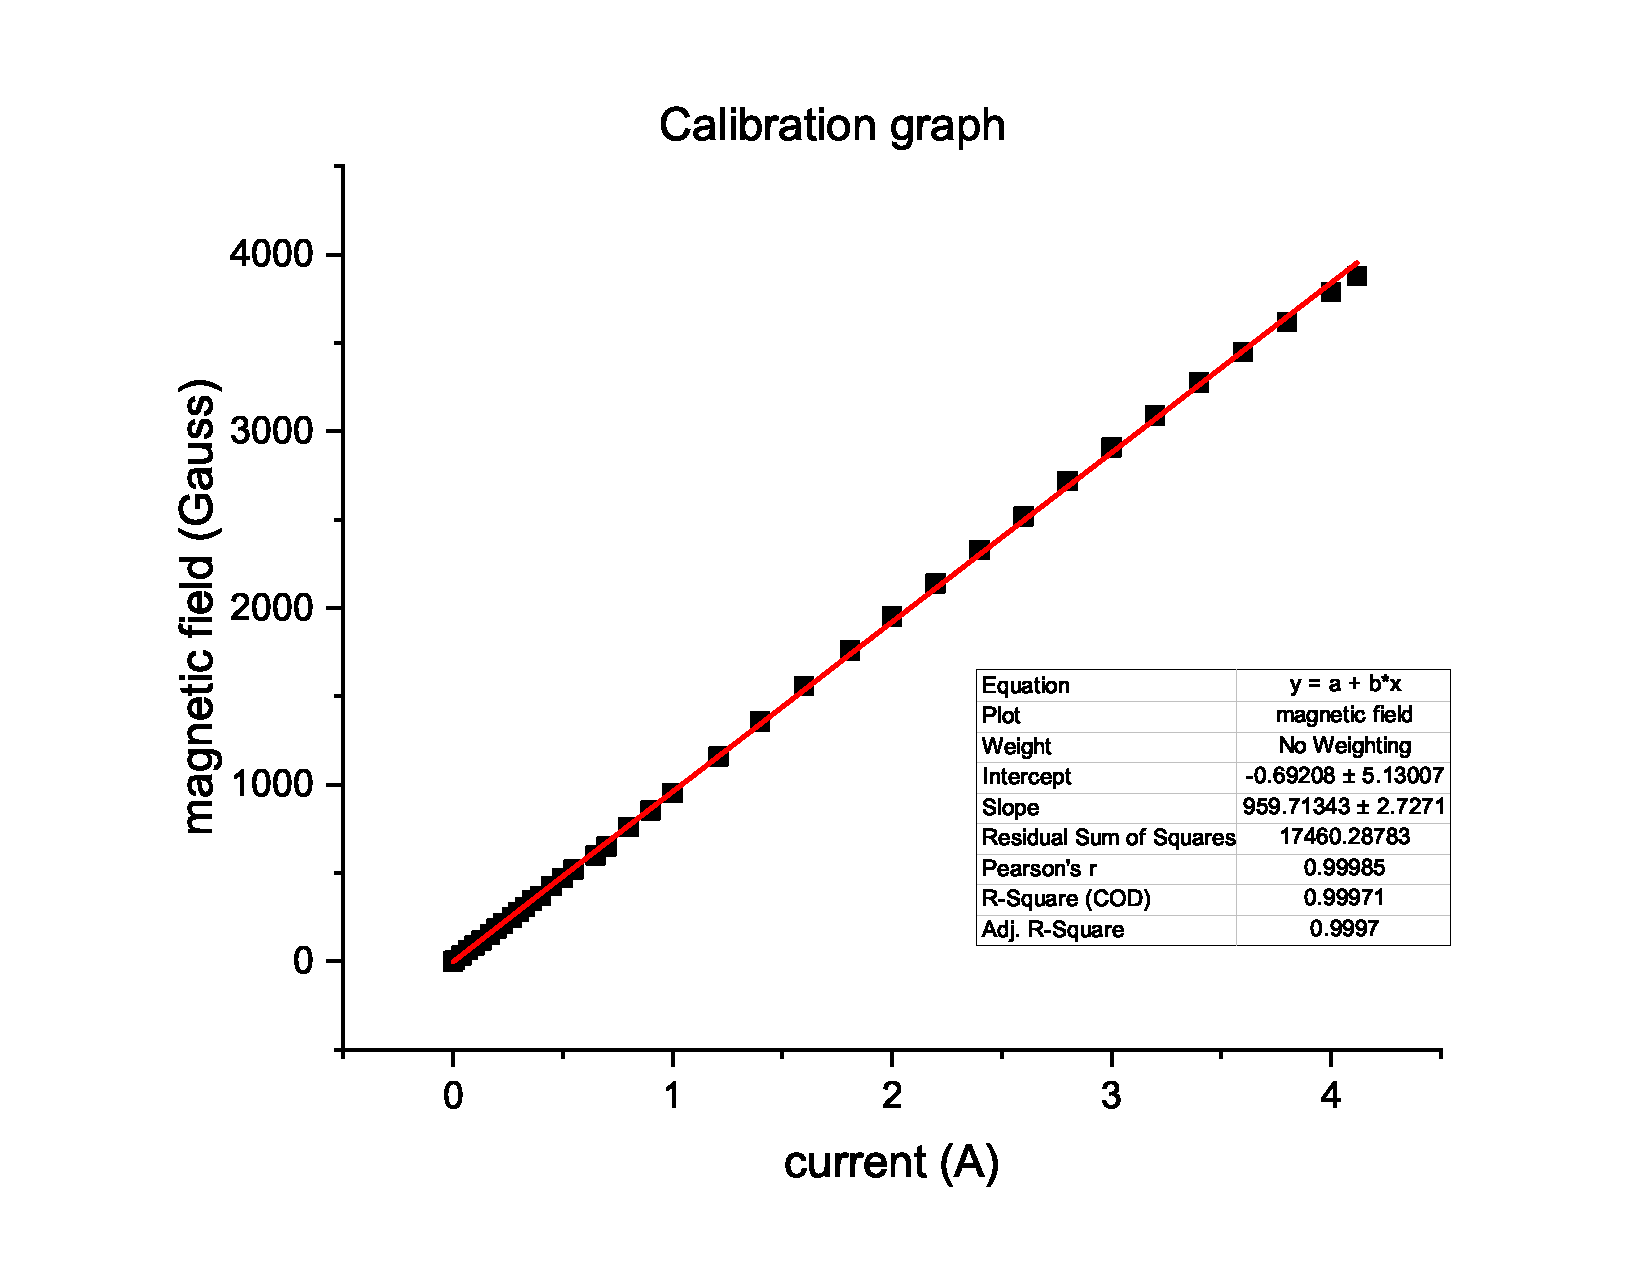
\includegraphics[width=0.8\columnwidth]{images/cal.eps}
			\caption{B vs I (coil current)}
			\label{graph:1}
		\end{figure}

	\subsection{Constant temperature}
		\subsubsection{Ge n-type}

			\begin{itemize}
				\item sample thickness = $t=0.5mm$
				\item coil current = $I=3.21A$
				\item $H=3277G$
			\end{itemize}

			We measured the Hall voltage at different probe current. The data is shown in Table \ref{tab:2}. The graph of Hall voltage vs probe current is shown in Fig \ref{graph:2}.

			from Graph \ref{graph:2}, we have $slope=\sfrac{V_y}{I_x}=-19.8$. Thus, using Equation \ref{eq:1} $ R_H=-3.02 cm^3 coulomb^{-1}$

			\begin{table}[H]
    \centering
    \begin{tabular}{|c|c|c|}
        \hline
        thickness & count & net count \\ \hline
        0         & 1216  & 204       \\ \hline
        0.6       & 853   & 783       \\ \hline
        0.12      & 706   & 636       \\ \hline
        0.18      & 504   & 434       \\ \hline
        0.24      & 420   & 350       \\ \hline
        0.3       & 311   & 241       \\ \hline
        0.36      & 222   & 152       \\ \hline
        0.42      & 199   & 129       \\ \hline
        0.48      & 168   & 98        \\ \hline
        0.54      & 145   & 75        \\ \hline
    \end{tabular}
    \label{tab:2}
    \caption{$\beta$ praticle counts for  $Tl^{204}$ in aluminium absorber}
\end{table}
			\begin{figure}[h]
				\centering
				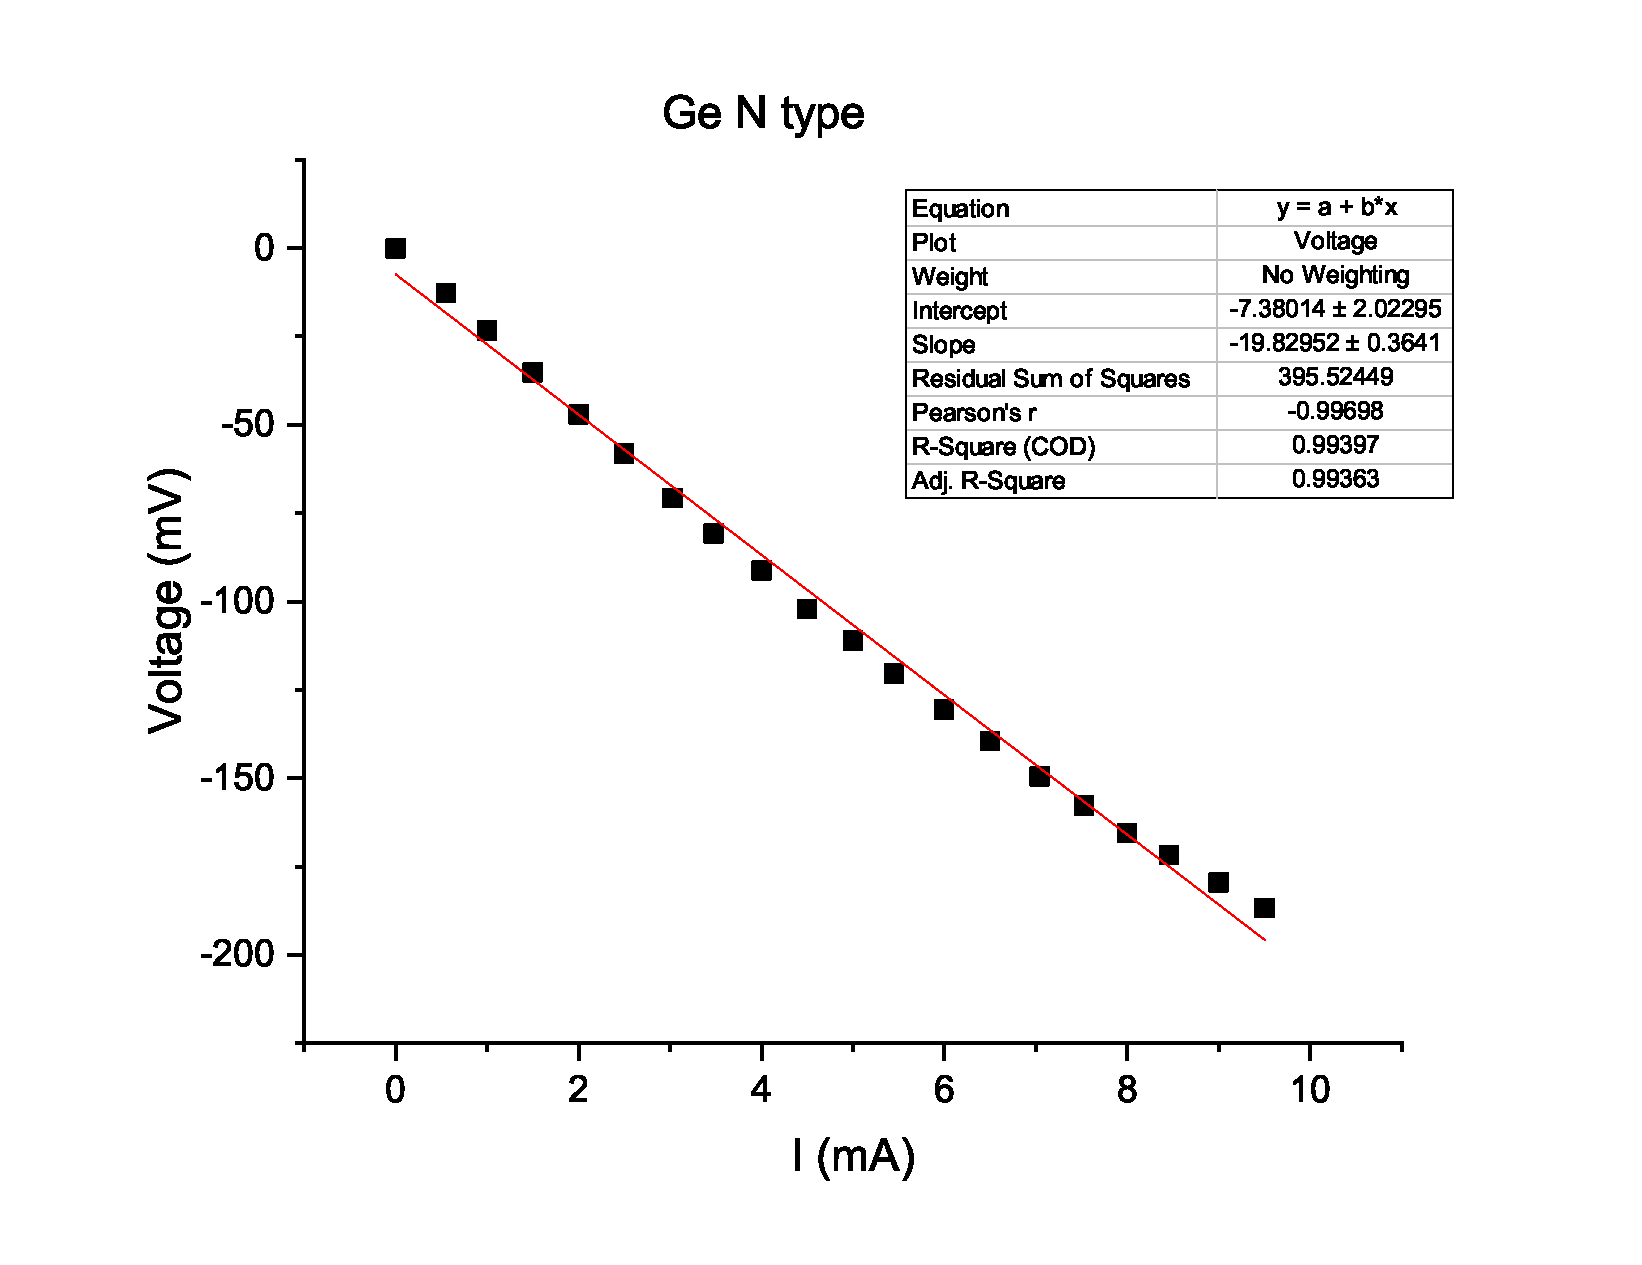
\includegraphics[width=0.9\columnwidth]{images/gen.eps}
				\caption{Hall voltage vs. probe current for Ge n-type}
				\label{graph:2}
			\end{figure}


		\subsubsection{Ge p-type}

			\begin{itemize}
				\item sample thickness = $t=0.5mm$
				\item coil current = $I=3.21A$
				\item $H=3277G$
			\end{itemize}
			
			% Please add the following required packages to your document preamble:
% \usepackage{graphicx}
\begin{table}[h]
    \centering
    \resizebox{0.75\columnwidth}{!}{%
    \begin{tabular}{|c|c|c|c|}
    \hline
    \textbf{I (mA)} & \textbf{\begin{tabular}[c]{@{}c@{}}Hall Voltage\\ (mV)\end{tabular}} & \textbf{\begin{tabular}[c]{@{}c@{}}Offset Voltage\\ (mV)\end{tabular}} & \textbf{\begin{tabular}[c]{@{}c@{}}Voltage\\ (mV)\end{tabular}} \\ \hline
    0.0 & 0 & 0 & 0 \\ \hline
    0.5 & 3.6 & -3.2 & 6.8 \\ \hline
    1.0 & 7.3 & -6.8 & 14.1 \\ \hline
    1.5 & 10.8 & -10.2 & 21.0 \\ \hline
    2.0 & 14.4 & -13.6 & 28.0 \\ \hline
    2.5 & 17.9 & -16.8 & 34.7 \\ \hline
    3.0 & 22.4 & -20.9 & 43.3 \\ \hline
    3.5 & 25.8 & -24.4 & 50.2 \\ \hline
    4.0 & 29.1 & -27.5 & 56.6 \\ \hline
    4.5 & 32.4 & -31.1 & 63.5 \\ \hline
    5.0 & 36.3 & -35.3 & 71.6 \\ \hline
    5.5 & 38.9 & -38.5 & 77.4 \\ \hline
    6.0 & 42.4 & -42.4 & 84.8 \\ \hline
    6.5 & 44.8 & -46.2 & 91.0 \\ \hline
    7.0 & 48.0 & -50.3 & 98.3 \\ \hline
    7.5 & 50.9 & -54.0 & 104.9 \\ \hline
    8.0 & 53.9 & -58.3 & 112.2 \\ \hline
    8.5 & 56.0 & -62.7 & 118.7 \\ \hline
    9.0 & 58.3 & -64.9 & 123.2 \\ \hline
    9.5 & 62.5 & -70.1 & 132.6 \\ \hline
    10.0 & 64.5 & -73.8 & 138.3 \\ \hline
    10.5 & 67.8 & -77.2 & 145.0 \\ \hline
    11.0 & 69.6 & -79.5 & 149.1 \\ \hline
    11.5 & 72.3 & -83.1 & 155.4 \\ \hline
    12.0 & 70.7 & -90.9 & 161.6 \\ \hline
    12.5 & 72.1 & -94.3 & 166.4 \\ \hline
    13.0 & 74.6 & -99.0 & 173.6 \\ \hline
    14.0 & 77.6 & -107.8 & 185.4 \\ \hline
    15.0 & 77.5 & -117.2 & 194.7 \\ \hline
    \end{tabular}%
    }
    \caption{Ge-P type hall voltage at different probe current}
    \label{tab:3}
\end{table}
			\begin{figure}[h]
				\centering
				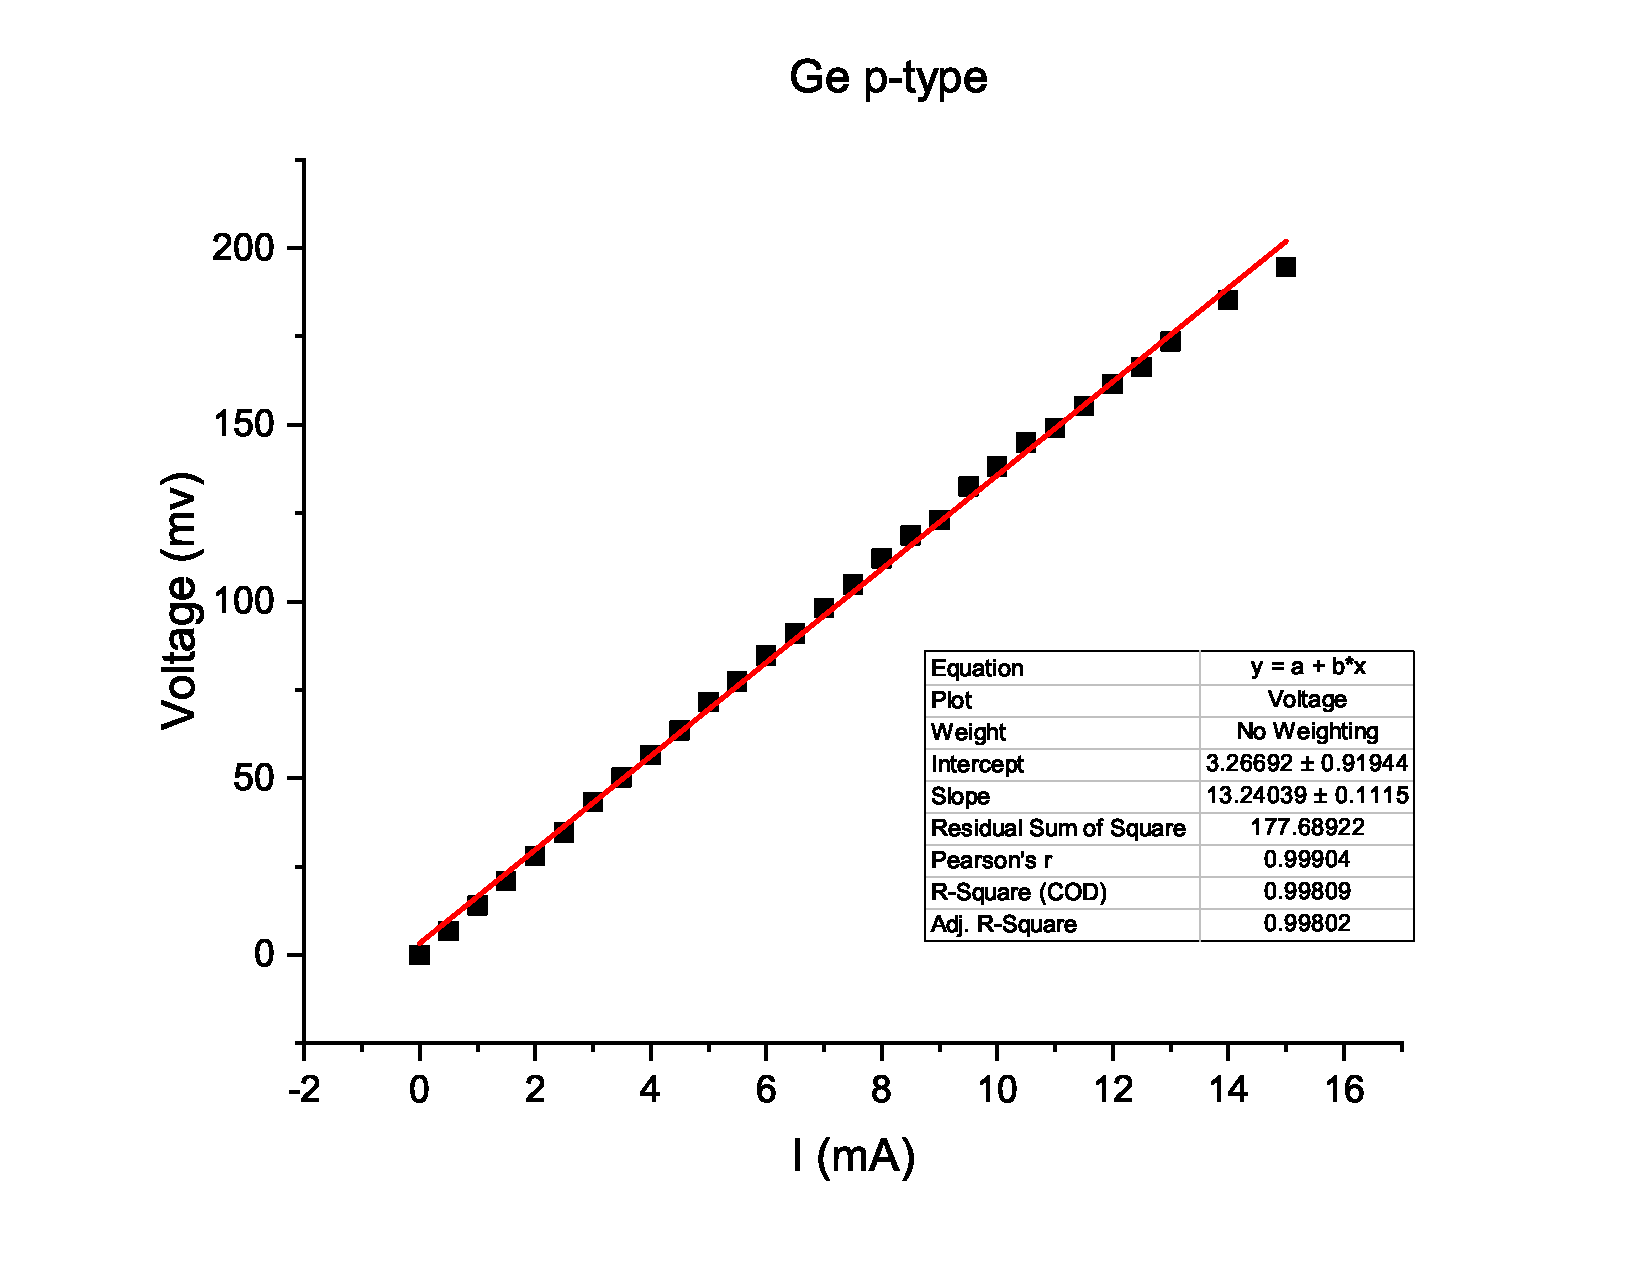
\includegraphics[width=0.9\columnwidth]{images/gep.eps}
				\caption{Hall voltage vs probe current for Ge p-type}
				\label{graph:3}
			\end{figure}

			We measured the Hall voltage at different probe current. The data is shown in Table \ref{tab:3}. The graph of Hall voltage vs probe current is shown in Fig \ref{graph:3}.

			from Graph \ref{graph:3}, we have $slope=\sfrac{V_y}{I_x}=-13.24$. Thus, using Equation \ref{eq:1} $ R_H=2.02 cm^3 coulomb^{-1}$
	\subsection{Temperature dependence of hall coefficient}
		\begin{itemize}
			\item sample thickness = $t=0.5mm$
			\item coil current = $I=3.07A$
			\item $H=2910G$
			\item probe current = $4.0 mA$
			\item Room temperature = $300K$
		\end{itemize}

		We measured the Hall voltage at different temperature. The data is shown in Table \ref{tab:4} and \ref{tab:5}. The graph of Hall coefficient vs temperature is shown in Fig \ref{graph}.

		\begin{figure}[h]
			\centering
			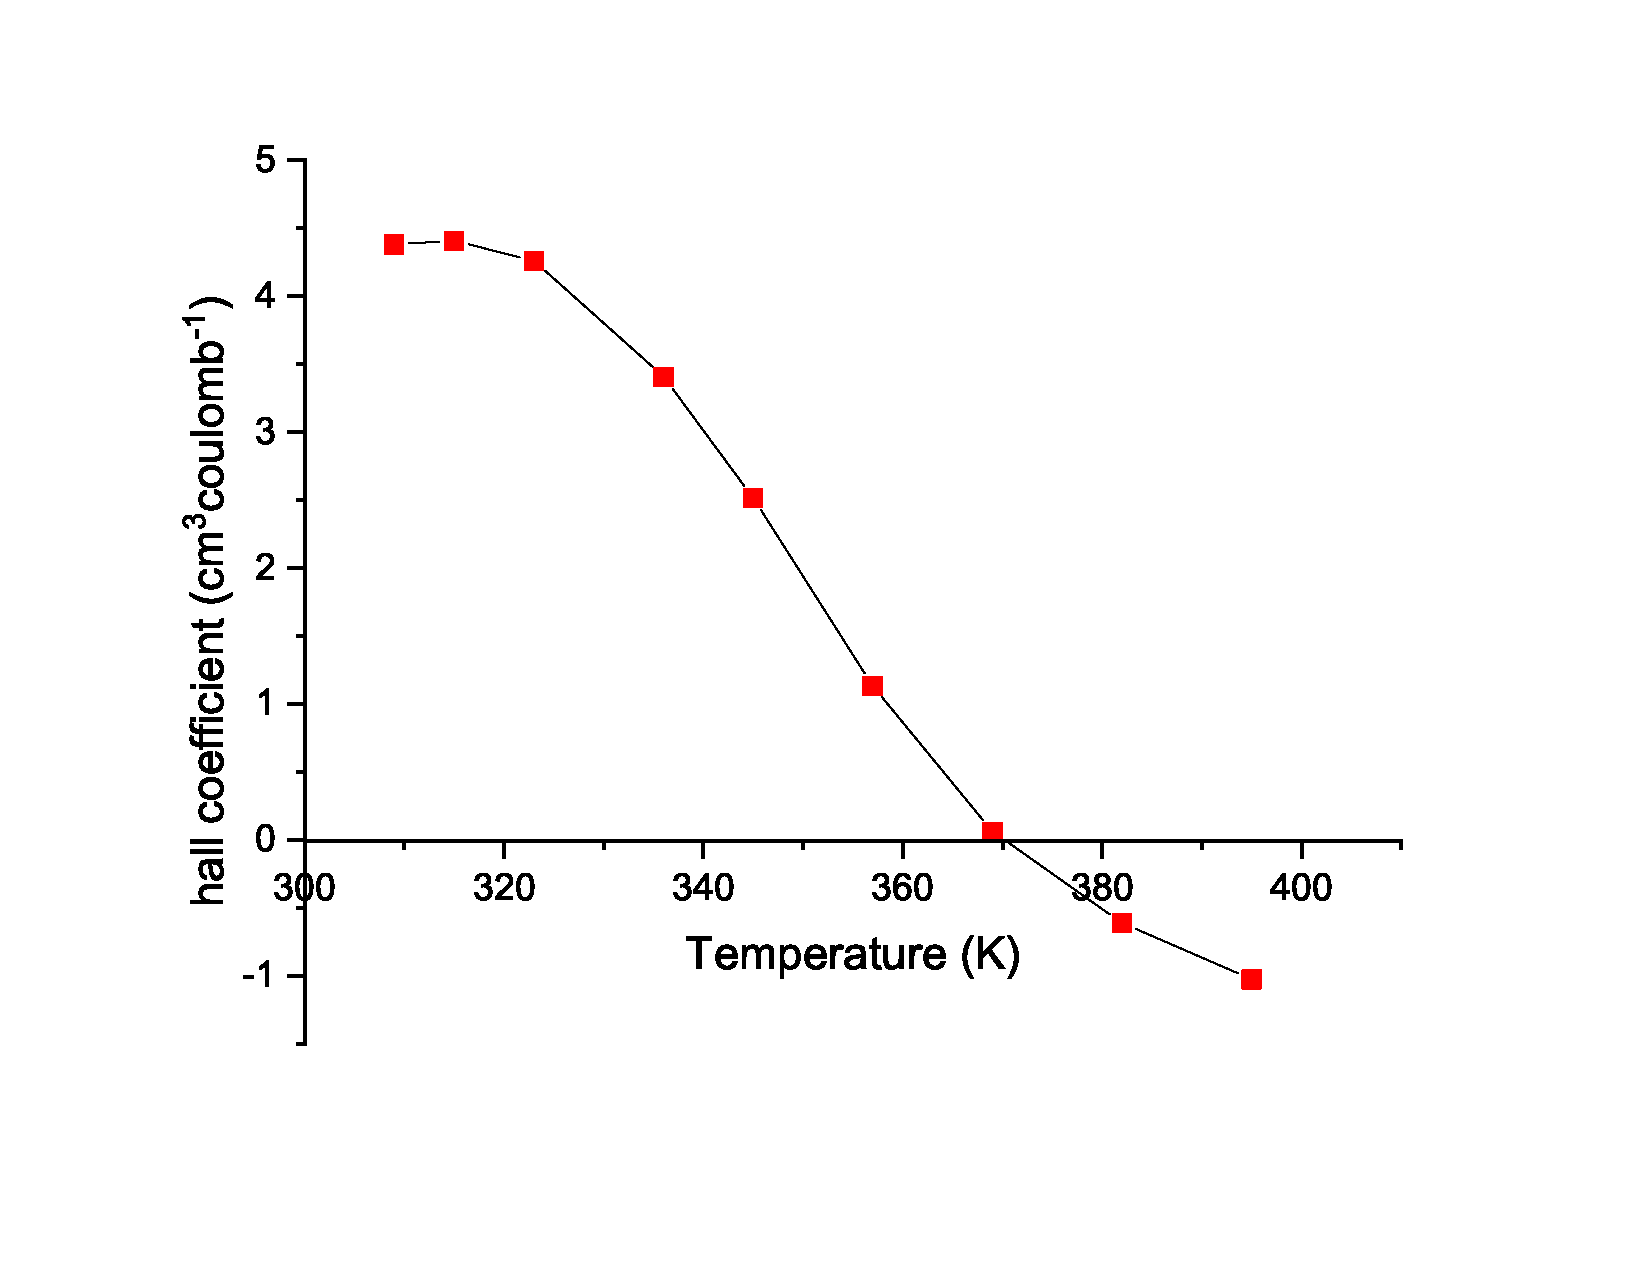
\includegraphics[width=0.9\columnwidth]{images/rh.eps}
			\caption{Hall coefficient vs. Temperature for Ge n-type}
			\label{graph}
		\end{figure}
		% Please add the following required packages to your document preamble:
% \usepackage{graphicx}
\begin{table}[]
	\centering
	\resizebox{\columnwidth}{!}{%
	\begin{tabular}{|c|c|c|c|c|}
	\hline
	\textbf{\begin{tabular}[c]{@{}c@{}}Heater\\ Current\end{tabular}} & \textbf{\begin{tabular}[c]{@{}c@{}}Thermal\\ EMF (mV)\end{tabular}} & \textbf{\begin{tabular}[c]{@{}c@{}}Hall\\ voltage (mV)\end{tabular}} & \textbf{\begin{tabular}[c]{@{}c@{}}Offset\\ voltage (mV)\end{tabular}} & \textbf{\begin{tabular}[c]{@{}c@{}}Voltage\\ (mV)\end{tabular}} \\ \hline
	304 & 0.35 & 145.4 & 43.4 & 102 \\ \hline
	405 & 0.6 & 146 & 43.4 & 102.6 \\ \hline
	501 & 0.91 & 142.6 & 43.4 & 99.2 \\ \hline
	605 & 1.43 & 122.7 & 43.4 & 79.3 \\ \hline
	706 & 1.8 & 102 & 43.4 & 58.6 \\ \hline
	802 & 2.32 & 69.8 & 43.4 & 26.4 \\ \hline
	900 & 2.81 & 44.8 & 43.4 & 1.4 \\ \hline
	1000 & 3.33 & 29.2 & 43.4 & -14.2 \\ \hline
	1100 & 3.9 & 19.5 & 43.4 & -23.9 \\ \hline
	\end{tabular}%
	}
	\caption{Hall voltage at different temperature}
	\label{tab:4}
\end{table}
		% Please add the following required packages to your document preamble:
% \usepackage{graphicx}
\begin{table}[h]
    \centering
    \resizebox{0.5\columnwidth}{!}{%
    \begin{tabular}{|c|c|}
    \hline
    \textbf{Temperature} & \textbf{Rh} \\ \hline
    309 & 4.3814433 \\ \hline
    315 & 4.40721649 \\ \hline
    323 & 4.26116838 \\ \hline
    336 & 3.40635739 \\ \hline
    345 & 2.51718213 \\ \hline
    357 & 1.13402062 \\ \hline
    369 & 0.06013746 \\ \hline
    382 & -0.60996564 \\ \hline
    395 & -1.0266323 \\ \hline
    \end{tabular}%
    }
    \caption{hall coefficient temperature dependance}
    \label{tab:5}
\end{table}
    \section{Error Analysis}
	We know that for a given relation:
	
	$$A = \frac{\prod n_i}{\prod d_i}$$
	
	For monitoring how the value of $A$ changes with \textbf{small} change in $n$ and $d$, we differentiate the equation and then divide it by the same equation. By doing this we get:
	
	$$\frac{dA}{A} = \sum\left(\frac{dn_i}{n_i}\right) - \sum\left(\frac{dd_i}{d_i}\right)$$

	So, for \textbf{Plateu Slope percent} in GM Characteristics we get:

	Error part in plateau slope percentage = $\frac{dslope}{slope} - \frac{dN}{N} = \frac{0.31}{1.99} - \frac{167}{4910} = 0.122$
	
	$\therefore$ plateu slope percentage = $(4.073 \pm 0.49)\%$

	For efficiency calculation, DPS was calculated from given value which were provided without any error information. So, we can assume that the error in DPS is negligible. Now, the standard deviation of the CPS in Cs is $0.194$ and in Tl is $0.023$. So, the value of effieciency with error bar is:

	\begin{itemize}
		\item Eff$_{Cs} = 31.62 \pm 0.549 \%$
		\item Eff$_{Tl} = 30.65 \pm 0.019 \%$
	\end{itemize}

	The error for counting statistics need not be calculated again because it had already been shown in \hyperref[graph:4]{Figure 6}

    \section{Conclusion}
	\begin{itemize}
		\item We conducted an experiment on Compton scattering of electrons, which involves the scattering of X-rays by free electrons.

		\item The observed data in our experiment shows that the intensity of scattered photons decreases as the scattering angle increases. This observation agrees with the Compton formula, which describes the energy transfer from photons to electrons in the scattering process.

		\item We also found that the energy of scattered photons decreases as the scattering angle increases, which again agrees with the Compton formula. This is because the energy of scattered photons is related to the energy lost by the electrons in the scattering process.

		\item Our experiment also revealed that the detector used in the experiment had different calibration factors for different materials. The calibration factor for brass was found to be approximately two times that of aluminum. This implies that for particular cross-sections, the relative intensity for brass is more than for aluminum.

		\item We calculated the rest mass of electrons in our experiment, but the result had a significant error. We think that this error can be minimized by taking precautions with the lead box used in the experiment. This suggests that our experiment can be improved by using better shielding to reduce unwanted background radiation and improve the accuracy of our measurements.

		\item Our experiment demonstrates that the Compton scattering process can be used to determine the rest mass of charged particles like electrons. By measuring the scattered photon energy and angle, along with the incident photon energy, it is possible to calculate the rest mass of the electron. This technique is widely used in experimental physics to measure the masses of particles.
	\end{itemize}

    

    % \bibliographystyle{apalike}
    \bibliography{ref.bib}
    \nocite{*}
\end{document}
